\section{ЗАЩИТА БАЗЫ ДАННЫХ ОТ НЕСАНКЦИОНИРОВАННОГО ДОСТУПА}

\subsection{Основные угрозы и уязвимости}

Основные угрозы, связанные с безопасностью веб-приложений, включают:

\begin{itemize}
    \item атаки на клиентов;
    \item утечка важных данных;
    \item НСД к приложению;
    \item НСД к функциональности или контенту;
    \item раскрытие конфигурационной информации;
    \item отказ в обслуживании;
    \item атаки на ресурсы;
    \item выполнение команд ОС на сервере.
\end{itemize}

На рисунке~\ref{fig:fig08} представлена доля угроз в процентном соотношении:

\begin{figure}
  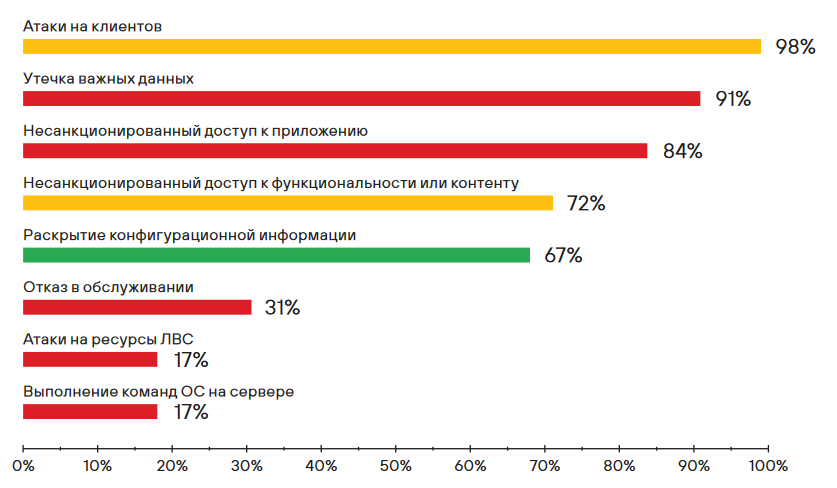
\includegraphics[scale=0.745]{inc/threats}
  \caption{Распространённые угрозы веб-приложений}
  \label{fig:fig08}
\end{figure}

Как можно заметить, утечка важных данных занимает второе место среди распространенных угроз на веб-приложения. Именно поэтому важно продумать систему защиты и хранения данных в БД.

Начиная с 2017 года актуальность атак на клиента возросла и возглавляет топ актуальных угроз. Атака вида – XSS (cross-site scripting) является каждой второй в списке атак. Сутью XSS уязвимости является возможность внедрения в веб-систему вредоносного кода и дальнейшего взаимодействия этого кода с серверами злоумышленника. Частным примером является SQL-инъекции.

SQL уязвимость основана на внедрении в запрос части произвольного SQL кода. Существует несколько способов применения SQL-инъекций использование числового входящего параметра и использование строкового входящего параметра.

Для предотвращения SQL-injection необходимо проводить правильную обработку пользовательского ввода, используя специальные методы для экранирования специальных символов и проверки вводимых данных. Например, можно использовать подготовленные запросы, которые разделяют SQL-код и данные, передаваемые в запросе, тем самым защищая приложение от выполнения злонамеренного кода.

Также важно следить за обновлением и патчингом используемых баз данных и их драйверов, чтобы избежать известных уязвимостей, которые могут быть использованы злоумышленниками для SQL-injection.

В целом, защита от SQL-инъекций требует аккуратности и внимательности в проектировании и разработке веб-приложений, а также постоянного мониторинга на наличие уязвимостей и проведения регулярных тестов на проникновение.




\subsection{Конфиденциальность персональных данных}

При разработке базы данных важно учитывать требования безопасности и конфиденциальности медицинской информации. Для этого могут быть приняты следующие меры:

\begin{itemize}
    \item шифрование данных: чувствительная медицинская информация, такая как персональные данные пациентов и медицинская история, должна быть зашифрована при хранении и передаче. Использование сильных шифровальных алгоритмов поможет защитить данные от несанкционированного доступа \cite{online11};
    \item многофакторная аутентификация: для обеспечения безопасности доступа к базе данных, особенно для медицинского персонала, следует реализовать многофакторную аутентификацию. Это требует предоставления нескольких форм идентификации, таких как пароль, биометрические данные или специальные токены, для подтверждения легитимности пользователя;
    \item управление доступом: реализация гибкой системы управления доступом поможет ограничить доступ к конфиденциальной информации только уполномоченному персоналу. Ролевая модель доступа может быть использована для определения прав доступа на основе ролей и ответственностей сотрудников;
    \item аудит и мониторинг: важно вести аудит и мониторинг доступа к базе данных для обнаружения и предотвращения несанкционированного доступа или неправомерной активности. Журналы доступа и системы мониторинга позволят выявить подозрительную активность и принять соответствующие меры;
    \item соответствие нормам и законодательству: разработка базы данных должна соответствовать применимым нормам и законодательству в области защиты персональных данных. Это включает в себя соблюдение правил по сбору, хранению, использованию и передаче медицинской информации;
    \item восстановление после катастрофы и резервное копирование: необходимо реализовать надежный план восстановления после катастрофы и резервного копирования, чтобы обеспечить доступность и целостность медицинской базы данных. Регулярные резервные копии должны выполняться, чтобы защитить от потери данных в случае сбоев системы, стихийных бедствий или кибератак. Также важно периодически тестировать процесс восстановления, чтобы убедиться в возможности точного и эффективного восстановления данных.
\end{itemize}

Анализируя вышеперечисленные пункты, можно сделать вывод, что обеспечение конфиденциальности хранения персональных данных является одним из ключевых вопросов, связанных с использованием цифровых медицинских карт и баз данных \cite{online6}.

Для обеспечения конфиденциальности данных необходимо проводить работу по защите информации и соблюдению законодательных требований. Организация должна предпринимать меры для защиты персональных данных пациентов, такие как использование паролей и шифрования данных. Кроме того, необходимо обучать медицинских работников основам информационной безопасности и контролировать доступ к информации.

Конфиденциальность хранения персональных данных пациентов - это важный аспект использования цифровых медицинских карт и организации должны принимать соответствующие меры для обеспечения безопасности информации и соблюдения законодательных требований.

PostgreSQL поддерживает множество функций для обеспечения безопасности данных, включая конфиденциальность хранения персональных данных.

Одним из ключевых механизмов для обеспечения конфиденциальности данных в PostgreSQL является использование различных методов шифрования, включая шифрование данных в пути и в покое, а также использование SSL для защиты соединений.

PostgreSQL также обеспечивает механизмы авторизации и аутентификации, которые позволяют контролировать доступ к базе данных и ее объектам, таким как таблицы и представления. Например, администраторы могут назначать различные роли и права доступа к объектам базы данных, что позволяет управлять доступом к конфиденциальным данным.

PostgreSQL также поддерживает аудиторскую функциональность, которая позволяет записывать действия пользователей в базе данных, такие как входы и выходы из системы, выполнение запросов и изменение данных. Это позволяет отслеживать и анализировать действия пользователей, чтобы обеспечить безопасность данных и защитить их от несанкционированного доступа.

В целом, PostgreSQL - это надежная и безопасная реляционная база данных, которая обеспечивает множество механизмов для защиты конфиденциальности данных, включая персональные данные пациентов.




\subsection{Использование имен пользователей, ролей и разрешений}

PostgreSQL обладает базовым механизмом защиты, включающим в себя идентификацию, аутентификацию и авторизацию. Идентификация – проверка на то, существует ли данный субъект, желающий воспользоваться данным ресурсом. Следующим шагом после идентификации следует аутентификация – проверка подлинности субъекта, в основном для этого используется паролевый метод. Конечным шагом является авторизация – предоставление необходимых прав субъекту или отказ в доступе к нужным ресурсам. Для реализации описанного механизма применяются учетные записи пользователей.

На рисунке~\ref{fig:fig09} представлено создание учетных записей для работников скорой медицинской помощи, а именно:

\begin{itemize}
    \item главный врач бригады - head\_physician;
    \item врач - doctor;
    \item фельдшер - paramedic;
    \item медсестра - nurse.
\end{itemize}

\begin{figure}
  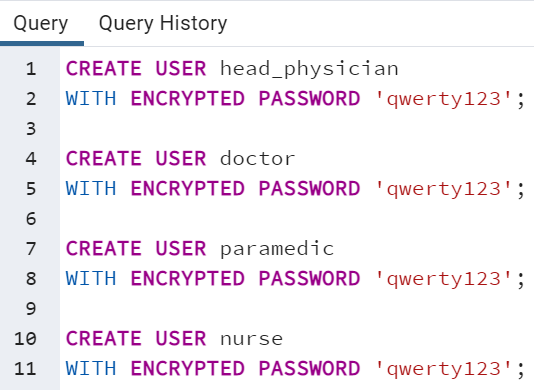
\includegraphics[scale=0.8]{inc/usernames}
  \caption{Создание учетных имен пользователей}
  \label{fig:fig09}
\end{figure}

Стоит остановиться на параметрах «CHECK\_EXPIRATION» и «CHECK\_POLICY», которые относятся к управлению паролями и их проверке при создании или изменении пользовательских данных. «CHECK\_EXPIRATION» отвечает за то, есть ли у пароля срок истечения, а «CHECK\_POLICY» определяет, должна ли использоваться паролевая политика. По умолчанию, проверка срока действия пароля и политики паролей включена в PostgreSQL, поэтому опции CHECK\_EXPIRATION и CHECK\_POLICY не нужно указывать.

Теперь нам нужно убедиться, что учетные имена пользователей и правда были созданы. Это продемонстрировано на рисунке~\ref{fig:fig10}.

\begin{figure}
  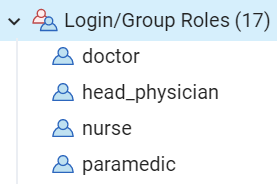
\includegraphics[scale=1]{inc/check_usernames}
  \caption{Проверка создания учетных имен пользователей}
  \label{fig:fig10}
\end{figure}

Определив учетные записи пользователей, остается лишь предоставить им необходимые разрешения, позволяющие взаимодействовать с БД. Можно отдельно каждому пользователю прописывать разрешения, но в данном случае это нецелесообразно – потому что фельдшера и медсестры должны быть одинаковые права, а у главврача и врача они такие же, только к тем правам добавляются еще другие. Выходом из этой ситуации являются роли. Роль – это объект БД, позволяющий объединять пользователей в единую группу с целью эффективного администрирования. Создание ролей и присоединение пользователей в роли продемонстрировано на рисунке~\ref{fig:fig11}.

\begin{figure}
  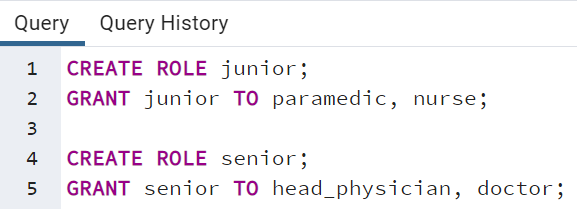
\includegraphics[scale=1]{inc/roles}
  \caption{Создание ролей и присоединение пользователей в роли}
  \label{fig:fig11}
\end{figure}

Проверим, находятся ли учетные записи в определенных ролях. Факт такого наличия изображен на рисунке~\ref{fig:fig12}.

\begin{figure}
  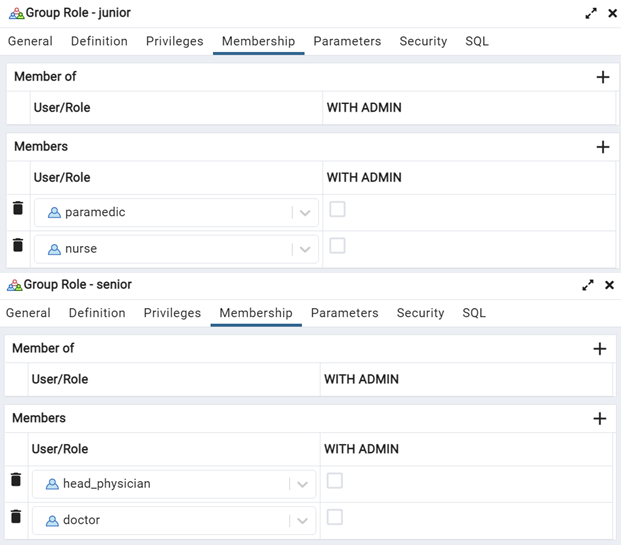
\includegraphics[scale=1.5]{inc/check_roles}
  \caption{Проверка на наличие пользователей в ролях}
  \label{fig:fig12}
\end{figure}

Создав роли для пользователей, нужно определить некоторые права, позволяющие манипулировать БД. Для этого в PostgreSQL предусмотрена возможность выдачи прав как отдельным пользователям, так и ролям.

Обозначим права, которые должны иметь роли. Роль «junior» должна иметь право на выборку всех таблиц существующей БД. Роль «senior» должна иметь право на выборку всех таблиц существующей БД, а также право на вставку, изменение и удаление значений всех таблиц, которые связаны с оказанием медицинской помощи и заполнением медкарты. На рисунке~\ref{fig:fig13} представлено присвоение ролям необходимых прав.

\begin{figure}
  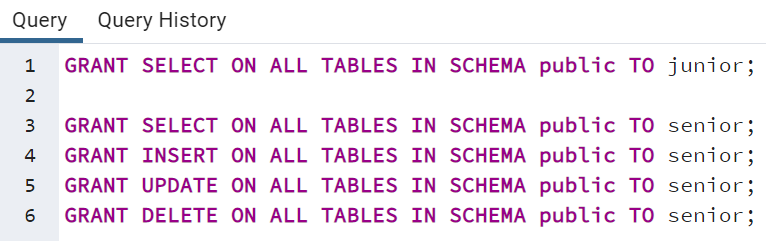
\includegraphics[scale=0.8]{inc/rights}
  \caption{Назначение прав ролям и пользователям}
  \label{fig:fig13}
\end{figure}

Стоит отметить еще одну возможность PostgreSQL. Для запрета на определенное право используется конструкция: «REVOKE action\_name ON object\_name FROM user\_name/role\_name;», при запрете права также может использоваться «CASCADE», это свойство наоборот запрещает некоторые права тем субъектам, которым оно выдавалось. Помимо выдачи и запрета прав есть третья возможность – отмена прав, она имеет следующий синтаксис: «REVOKE action\_name ON object\_name FROM user\_name/role\_name [CASCADE];», свойство «CASCADE» используется для отмены прав у тех субъектов, которым данный пользователь выдал. Стоит обратить внимание, что для использования команды REVOKE в PostgreSQL необходимо иметь соответствующие привилегии администратора базы данных.

pgAdmin также позволяет просмотреть права ролей у каждой таблицы. На рисунке~\ref{fig:fig14} изображены предоставленные права к таблице «Медикаменты».

\begin{figure}
  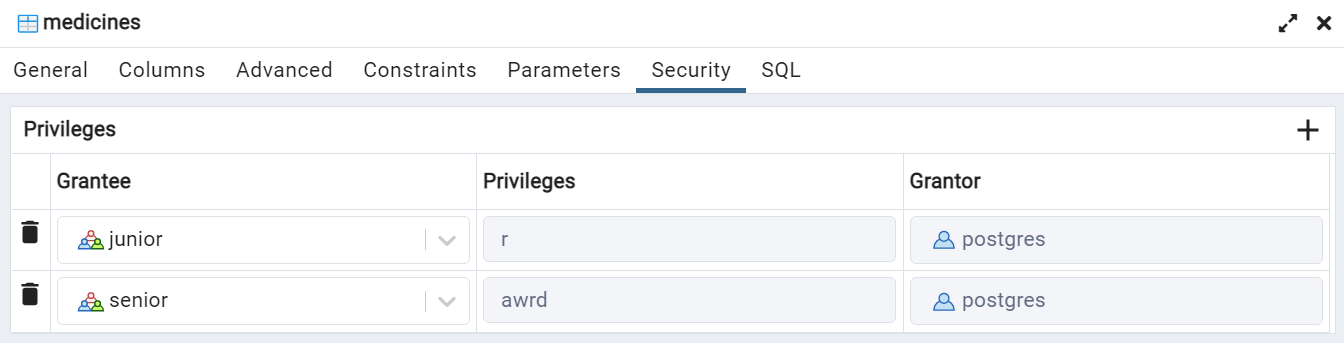
\includegraphics[scale=0.46]{inc/rights_tables}
  \caption{Проверка ролей на их возможные права в таблице}
  \label{fig:fig14}
\end{figure}





\subsection{Шифрование базы данных}

Вторым базовым механизмом защиты, реализующимся в PostgreSQL, от НСД является шифрование БД. Шифрование – это преобразование исходной информацию в данные, которые теряют иной смысл, не зная секретного слова или алгоритма, преобразовывающие данные обратно в смысловую информацию.

Самый популярный способ зашифровать информацию, хранящуюся в БД – это прозрачное шифрование данных. Преимущество такого вида шифрования заключается в том, что конечные пользователи могут даже и не знать, что применяется защита информации.

Прозрачное шифрование, также известное как шифрование в режиме реального времени, представляет собой способ защиты данных, при котором шифрование и расшифровка осуществляются автоматически без участия пользователя. Этот метод основан на работе специального драйвера, который функционирует в фоновом режиме и следит за всеми операциями с данными. Его главная цель заключается в предотвращении атак, направленных на получение данных путем обхода операционной системы, например, через загрузку из другой ОС или использование альтернативных методов.

Перед тем, как перейти к шифрованию, следует, на всякий случай, сделать резервную копию БД. Для этого следует включить pgAgen.

Затем выбираем нужную БД, вызываем контекстное меню, в нем выбираем опцию «создать резервную копию».

Создав резервную копию БД, можно приступать к процессу шифрования. Этот процесс происходит в несколько этапов:

\begin{itemize}
    \item создание главного ключа БД;
    \item создание сертификата;
    \item создание ключа шифрования;
    \item запуск процесса шифрования;
    \item проверка состояния шифрования.
\end{itemize}

Главный ключ БД – это ключ, который применяется для шифрования других ключей, использующихся для реализации шифрования в БД. Для его создания применяется следующая конструкция: «CREATE MASTER KEY ENCRYPTION BY PASSWORD 'password';».

Следующим шагом будет создание сертификата. Сертификат – это объект безопасности, имеющий подпись. Этот объект хранит в себе ключи шифрования. Для создания данного объекта применяется следующая конструкция: «CREATE CERTIFICATE name\_db\_and\_cert WITH SUBJECT 'description';».

Последним подготовительным этапом перед началом шифрования БД является создание ключа шифрования. Именно этим ключом будет происходить шифрование БД, а сам ключ будет находиться в сертификате, созданном заранее. Для его создания требуется применять следующий шаблон: «CREATE DATABASE ENCRYPTION KEY WITH ALGORITHM = AES\_128 ENCRYPTION BY SERVER CERTIFICATE cert\_name;».

Следующий шаг является необязательным, но его желательно выполнять. При создании главного ключа, сертификата и ключа шифрования рекомендуется создание резервных копий этих объектов безопасности. Для создания резервной копии ключа шифрования можно использовать команду pg\_dump, которая создаст резервную копию всей базы данных, включая ключи шифрования: «pg\_dump dbname > backup\_file\_name;».

Все объекты безопасности проинициализированы, также для критических объектов были созданы резервные копии. Теперь можно приступать к шифрованию БД. Для начала данного процесса используется следующий пакет команд: «UPDATE table\_name SET column\_name = pgp\_sym\_encrypt(column\_name, 'key\_password');».

Осталось лишь проверить, работает ли ключ шифрования для БД. Для этого используются системные БД «pg\_database\_encryption». Нас интересует столбец is\_encrypted, если шифрование завершилось успешно, то столбец принимает значение 1.

Но, сказать честно, нас мало интересует сквозное шифрование всей БД. Ведь сквозное шифрование всей базы данных может иметь несколько негативных аспектов:

\begin{itemize}
    \item высокая нагрузка на производительность: Шифрование и дешифрование больших объемов данных может быть ресурсоемким процессом, что может замедлить операции чтения и записи в базе данных. Это особенно актуально для приложений с высокой нагрузкой или большим количеством одновременных пользователей;
    \item ограничения по поиску и сортировке: Шифрованные данные нельзя эффективно искать или сортировать без их предварительного расшифрования. Если в базе данных необходимо выполнять сложные операции поиска или агрегации данных, то сквозное шифрование может существенно затруднить выполнение этих операций;
    \item управление ключами: Для сквозного шифрования необходимо использовать сильные шифровальные ключи, их генерацию, хранение и управление. Ключи должны быть доступны для расшифровки данных, что может представлять риск безопасности, особенно если ключи утекают или попадают в неправильные руки;
    \item затрудненная администрация: Сквозное шифрование требует дополнительного управления и конфигурации в базе данных и приложениях. Это может усложнить администрирование базы данных и требовать дополнительных усилий для поддержки и масштабирования системы;
    \item ограниченные возможности обработки данных: Шифрование данных делает их недоступными для анализа, обработки и использования в алгоритмах машинного обучения или других высокоуровневых операциях, которые требуют доступа к исходным данным.
\end{itemize}

Вместо сквозного шифрования всей базы данных может быть целесообразнее использовать частичное шифрование, где шифруются только конкретные конфиденциальные данные или поля, сохраняя остальные данные в незашифрованном виде. Это позволяет более гибко балансировать безопасность и производительность системы. Именно так мы и поступим. Будем шифровать только те данные, которые могут определенно точно идентифицировать личность человека.

Воспользуемся модулем pgcrypto для симметричного шифрования выборочных данных. Но для начала убедимся, что модуль установлен. На рисунке~\ref{fig:fig15} можно видеть, что у нас все готово к работе.

\begin{figure}
  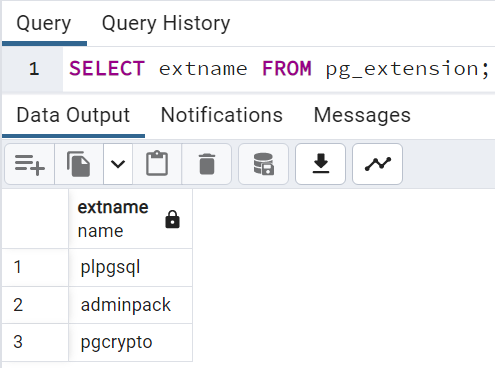
\includegraphics[scale=0.52]{inc/pgcrypto}
  \caption{Проверка наличия модуля pgcrypto}
  \label{fig:fig15}
\end{figure}

Можно шифровать и расшифровывать столбцы в таблицах в созданной БД:

\begin{itemize}
    \item для шифрования используется следующий шаблон: «UPDATE mytable SET mycolumn = pgp\_sym\_encrypt(mycolumn, 'mysecretkey');»;
    \item для расшифрования используется следующий шаблон: «SELECT pgp\_sym\_decrypt(mycolumn, 'mysecretkey') AS decrypted\_data FROM mytable;».
\end{itemize}

На рисунке~\ref{fig:fig16} приведены данные в чистом виде без шифрования.

\begin{figure}
  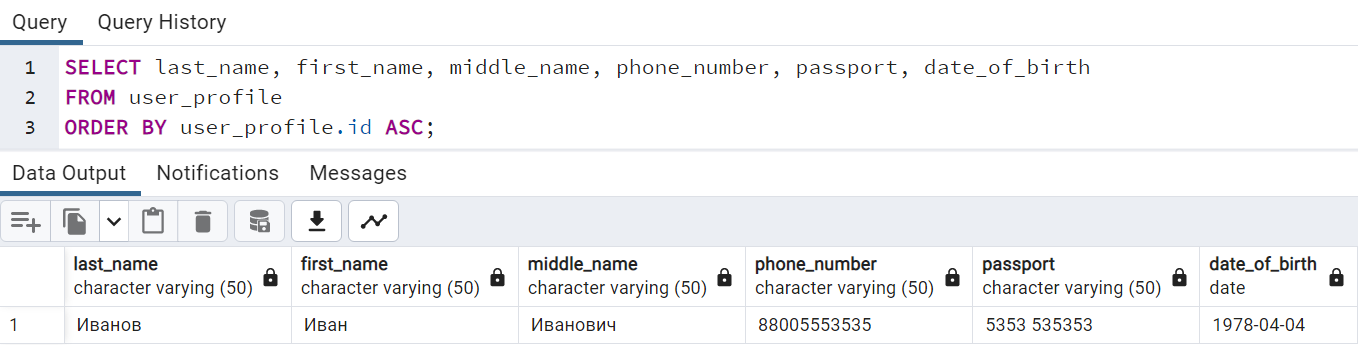
\includegraphics[scale=0.456]{inc/table_user_profile}
  \caption{Изначальные данные таблицы user\_profile}
  \label{fig:fig16}
\end{figure}

На рисунке~\ref{fig:fig17} представлен пример того, как шифруются некоторые столбцы.

\begin{figure}
  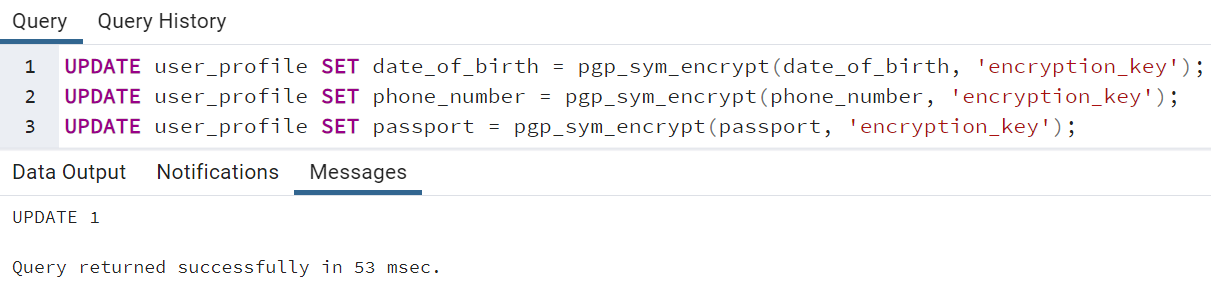
\includegraphics[scale=0.51]{inc/encryption}
  \caption{Шифрование некоторых данные таблицы user\_profile}
  \label{fig:fig17}
\end{figure}

Теперь убедимся, что наши данные и правда были зашифрованы. Это можно увидеть на рисунке~\ref{fig:fig18}.

\begin{figure}
  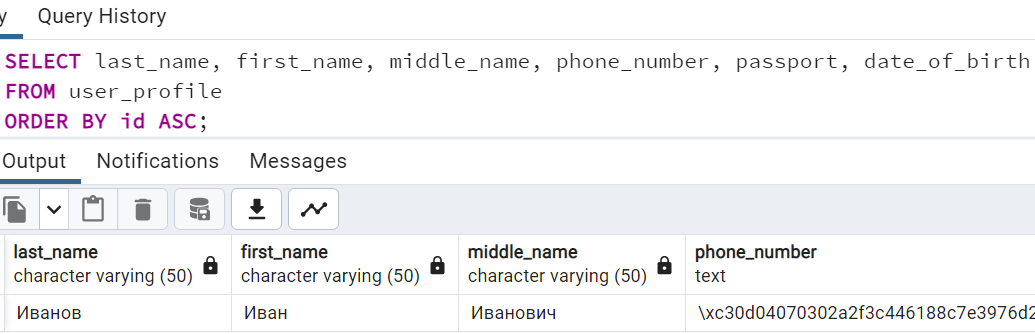
\includegraphics[scale=0.6]{inc/encrypted_table}
  \caption{Проверка шифрования некоторых данных таблицы user\_profile}
  \label{fig:fig18}
\end{figure}

На рисунке~\ref{fig:fig18} видно, что столбец с паспортными данными успешно зашифрован и можно не переживать за конфиденциальность хранения персональных данных. Но что теперь делать, нужно же не только хранить, но и получать данные из таблицы. Для этого при выполнении запроса вызывается функция расшифрования с тем самым ключом, который использовался при шифровании. На рисунке~\ref{fig:fig19} продемонстрирован запрос на получения данных в зашифрованного столбца с процессом расшифрования по ходу выполнения.

\begin{figure}
  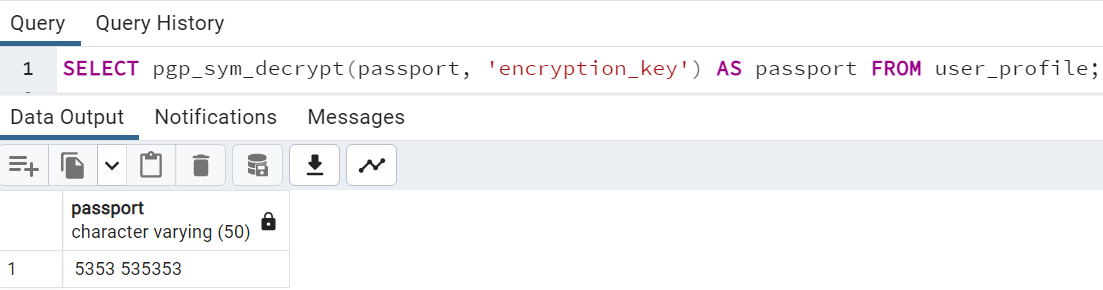
\includegraphics[scale=0.847]{inc/decryption}
  \caption{Получение данных зашифрованного столбца с расшифрованием в процессе выполнения запроса}
  \label{fig:fig19}
\end{figure}

В конечном итоге, после расшифрования всех данных, мы получим идентичные данные, что были до процесса шифрования. На рисунке~\ref{fig:fig20} можно увидеть, что целостность данных не была нарушена после процессов шифрования и дешифрования данных.

\begin{figure}
  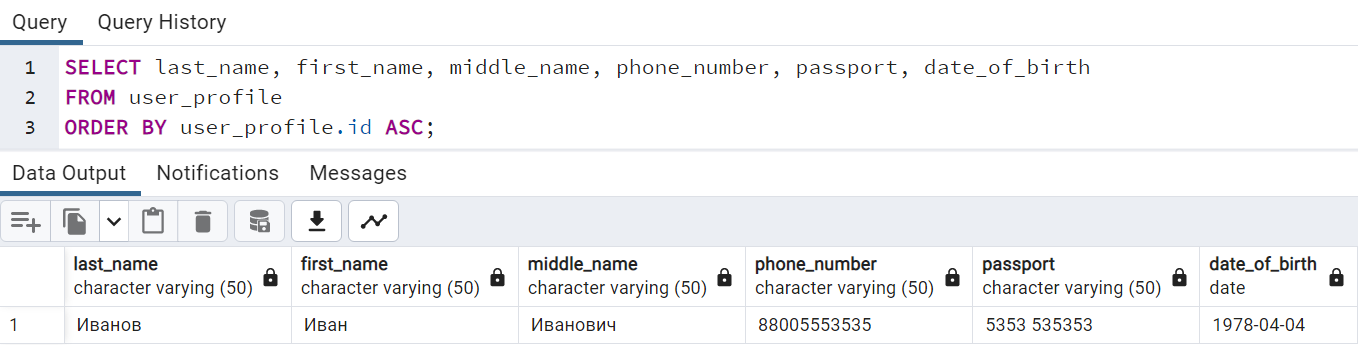
\includegraphics[scale=0.456]{inc/table_user_profile}
  \caption{Подтверждение целостности данных}
  \label{fig:fig20}
\end{figure}



\subsection{Порты}

Порт – это некоторое идентифицирующее число от 1 до 65535, позволяющее протоколам взаимодействовать друг с другом на транспортном уровне модели OSI.

На самом деле, у PostgreSQL сервера по умолчанию установлен только один порт, и это TCP порт.

PostgreSQL использует TCP/IP для обмена данными между клиентами и сервером. По умолчанию, порт TCP для PostgreSQL установлен на 5432. TCP 5432: database engine, используется для подключения к СУБД. Этот порт можно изменить при настройке сервера \cite{online7}.

Несмотря на то, что UDP не используется для коммуникации между клиентами и сервером PostgreSQL, есть несколько расширений, таких как pgpool-II, которые могут использовать UDP для взаимодействия между серверами PostgreSQL.

Таким образом, можно сказать, что PostgreSQL сервер по умолчанию использует только один порт TCP для обмена данными между клиентами и сервером.

Хорошей практикой является смена портов на другие, чтобы при случае атаки порты пришлось перебирать методом грубого подбора, а не использовать установленные по умолчанию. По данным IANA, порты 834-846 являются свободными, поэтому мы их можем использовать.

Для изменения порта, используемого PostgreSQL, можно внести изменения в конфигурационный файл postgresql.conf, который находится в каталоге данных PostgreSQL.

В файле postgresql.conf необходимо изменить параметр port на желаемое значение порта. Например, если вы хотите использовать порт 840 вместо стандартного порта 5432, необходимо изменить строку: port = 5432 на port = 840. После этого нужно перезапустить PostgreSQL, чтобы изменения вступили в силу.

Также можно использовать параметр командной строки -p при запуске сервера PostgreSQL для указания порта. Например, чтобы запустить PostgreSQL на порту 840, необходимо использовать команду: postgres -p 840, но в этом случае необходимо убедиться, что порт 840 свободен и не используется другим приложением на сервере.

Помимо смены порта, слушающий входящие соединения, можно отключить PostgreSQL Server. PostgreSQL Server – это одна из служб PostgreSQL, отвечающая за прослушивание запросов. Если эту службу отменить, то для установления соединения придется явно указывать номер порта, что обеспечивает дополнительную безопасность. Для остановки этой службы требуется просто ввести sudo systemctl stop postgresql в командной строке.



\subsection{Брандмауэр}

Брандмауэр – это программный межсетевой экран, имеющийся в ОС Windows. В свою очередь межсетевой экран – это элемент локальной сети, осуществляющий мониторинг активности в данной сети, а именно фильтрацию сетевого трафика по заранее описанным правилам. PostgreSQL Server функционирует на ОС Windows, поэтому рекомендуется использовать Брандмауэр вместе с программно-аппаратным межсетевым экраном. Такое сочетание позволяет повысить уровень защищенности за счёт использования дополнительных механизмов защиты информации. Также Брандмауэр обеспечивает не только защищенность от НСД, но и от поступающего вредоносного трафика в принципе.

Как было описано выше, межсетевой экран анализирует сетевой трафик и отклоняет его, если он считается подозрительным. Выше мы поменяли стандартный TCP/UDP порт 5432 на 840, теперь нужно объявить правило в межсетевом экране, что публичная сеть не может ссылаться на этот порт. Для этого заходим в Монитор Брандмауэра Защитника Windows в режиме повышенной безопасности и создадим новое правило. Далее определяем, что правило создается для порта, затем вписываем наш нужный порт, после этого разрешаем подключение, после этого исключаем публичный доступ, и в конце сохраняем наше правило.


\bigbreak
\textbf{Выводы по разделу}
\bigbreak

В этом разделе разбирались аспекты, связанные с безопасностью. Для защиты от НСД внутренними средствами PostgreSQL была реализована авторизация пользователей, а также им были назначены необходимые минимальные права для работы с БД, что позволило осуществить легитимный доступ к информации. Для повышения конфиденциальности информации использовалось шифрование информации на уровне столбцов при помощи библиотеки pgcrypto. Кроме того, при помощи шифрования файлы БД были защищены от кражи на физических носителях. А изменение портов и использование Брандмауэра позволило защититься на сетевом уровне. В совокупности была выполнена задача определения защитных мер БД.